\section{Results}
\label{sec:results}

The results are presented in the following order: validity of the proxy (RQ2), behavior of the two searches and the test comparison of the three arms (RQ1), and the change from studio to real-world and Indian photographs (RQ3). Their interpretation is taken up in Section~\ref{sec:discussion}.

\subsection{Proxy Validity}
\label{subsec:res-proxy}

The proxy passed the check that had been defined before the \genone searches (Section~\ref{subsec:proxy}). The Spearman rank correlation between the proxy scores and the 40-epoch medium scores is $\rho = 0.976$ ($n = 8$), which is much higher than the pass threshold of 0.6 (Table~\ref{tab:proxy} and Fig.~\ref{fig:proxy}). The two rankings are identical except that the neighboring settings lhs3 and lhs5 are interchanged. The same four settings are at the top of both rankings, and in both the defaults come second after lhs4. However, the medium scores of these four settings are within 0.026 of one another. The proxy is therefore much better at separating poor settings from good ones than at ordering the good ones among themselves.

\begin{table}[!t]
\centering
\caption{Proxy-Validity Check (\genone, Validation \mapfifty)}
\label{tab:proxy}
\footnotesize
\begin{tabular}{@{}lcccc@{}}
\toprule
Setting & Proxy & Rank & Medium & Rank \\
\midrule
lhs1 & 0.08687 & 1 & 0.28423 & 1 \\
lhs2 & 0.23077 & 2 & 0.49451 & 2 \\
lhs3 & 0.29495 & 3 & 0.56712 & 4 \\
lhs5 & 0.30186 & 4 & 0.55195 & 3 \\
lhs7 & 0.37560 & 5 & 0.61246 & 5 \\
lhs6 & 0.44285 & 6 & 0.62161 & 6 \\
Defaults & 0.47648 & 7 & 0.62884 & 7 \\
lhs4 & 0.49547 & 8 & 0.63839 & 8 \\
\midrule
\multicolumn{5}{@{}l@{}}{Spearman $\rho = 0.976$, $n = 8$; pass threshold $\rho \ge 0.6$} \\
\bottomrule
\end{tabular}
\\[2pt]
\parbox{\columnwidth}{\footnotesize Proxy: 12 epochs on the stratified 40\% training subset. Medium: 40 epochs on the full training split. Both at 416~px; rank 1 is the lowest score. lhs1--lhs7 are the Latin hypercube settings.}
\end{table}

\begin{figure}[!t]
\centering
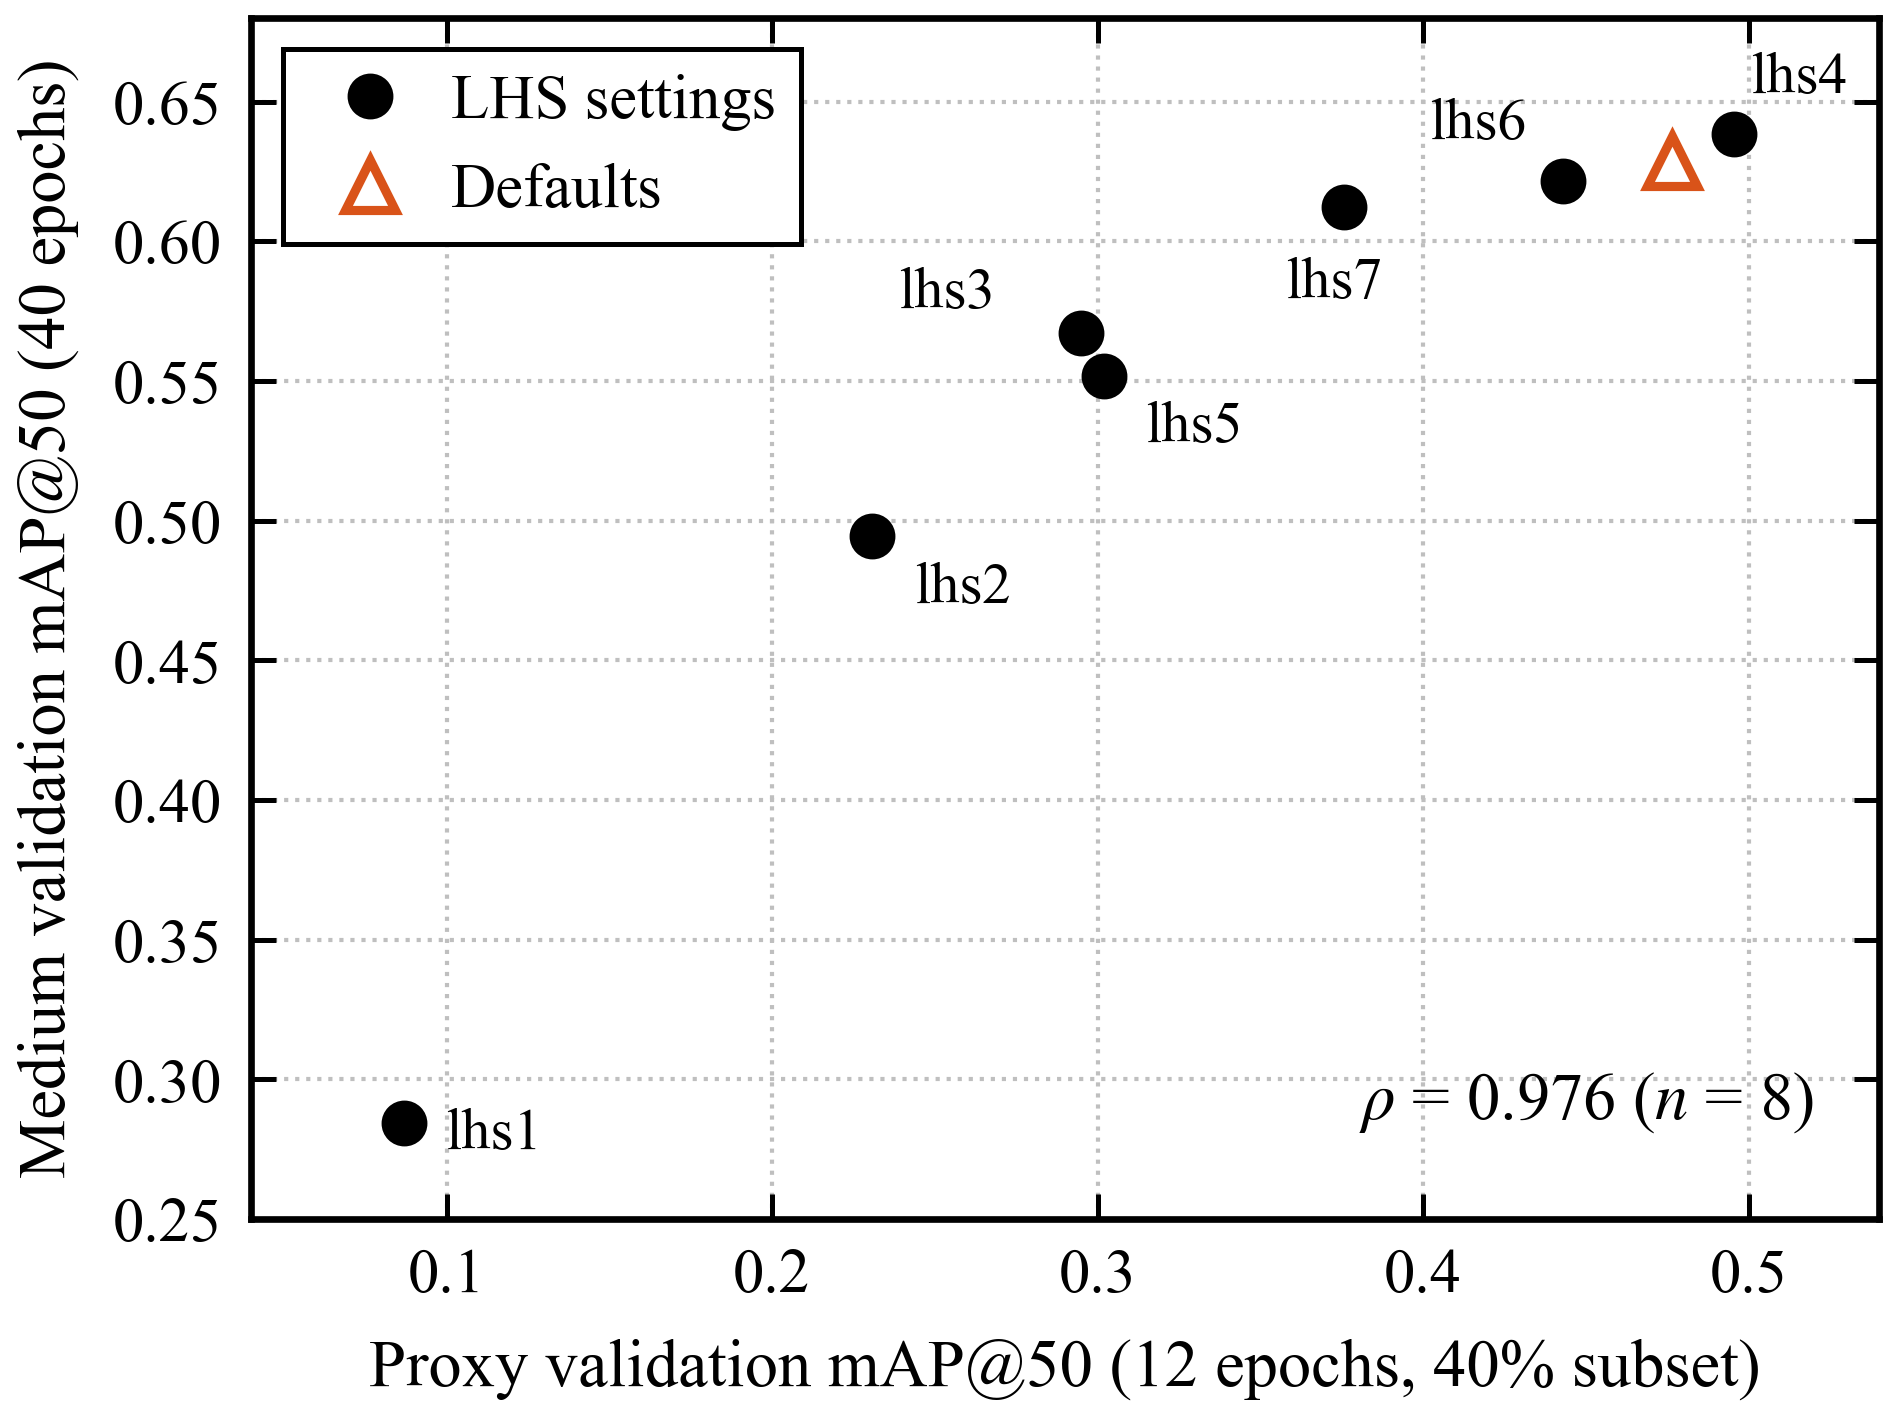
\includegraphics[width=\columnwidth]{r_proxy.png}
\caption{Proxy versus medium validation \mapfifty of the eight settings used in the \genone proxy-validity check. The two rankings agree except for the neighboring pair lhs3 and lhs5.}
\label{fig:proxy}
\end{figure}

A second, indirect check is possible because some configurations were evaluated in both generations. As the seeds and the search space were the same, random search sampled the same 32 configurations in \genone and \gentwo. In PSO, the positions depend on the fitness only through the personal and global bests. These coincided long enough for the swarm to visit identical positions in rounds 1--3 (24 evaluations), but not in round~4. For these repeated configurations, the Spearman correlation between the proxy scores of the two generations is 0.991 for random search and 0.892 for PSO, computed from the four search logs. It should be kept in mind that this compares one proxy with another proxy and not a proxy with longer training. It shows that the two generations order the settings similarly, but it is not a substitute for a proxy-validity check on \gentwo.

\subsection{Search Behavior}
\label{subsec:res-search}

Fig.~\ref{fig:convergence} plots all proxy evaluations along with the best score obtained so far. In \genone, random search reached its best setting (proxy \mapfifty of 0.4995) at the second evaluation itself and did not improve afterwards. PSO improved gradually, from 0.4894 after round~1 to 0.4942 after round~3 and 0.4953 in round~4 (evaluation 27). The swarm converged as expected: the mean score per round increased from 0.393 to 0.423, 0.450 and 0.482, while the standard deviation within a round decreased from 0.122 to 0.088, 0.047 and 0.011. The defaults obtained 0.4765 on the same proxy, which is higher than 28 of the 32 evaluations of random search and 21 of the 32 evaluations of PSO. The two winners are separated by only 0.0042, and lhs4 from the proxy check (0.4955) falls between them. Interestingly, the four search winners of the two generations all have an initial learning rate (0.0025 to 0.0070) below the default value of 0.01.

\begin{figure*}[!t]
\centering
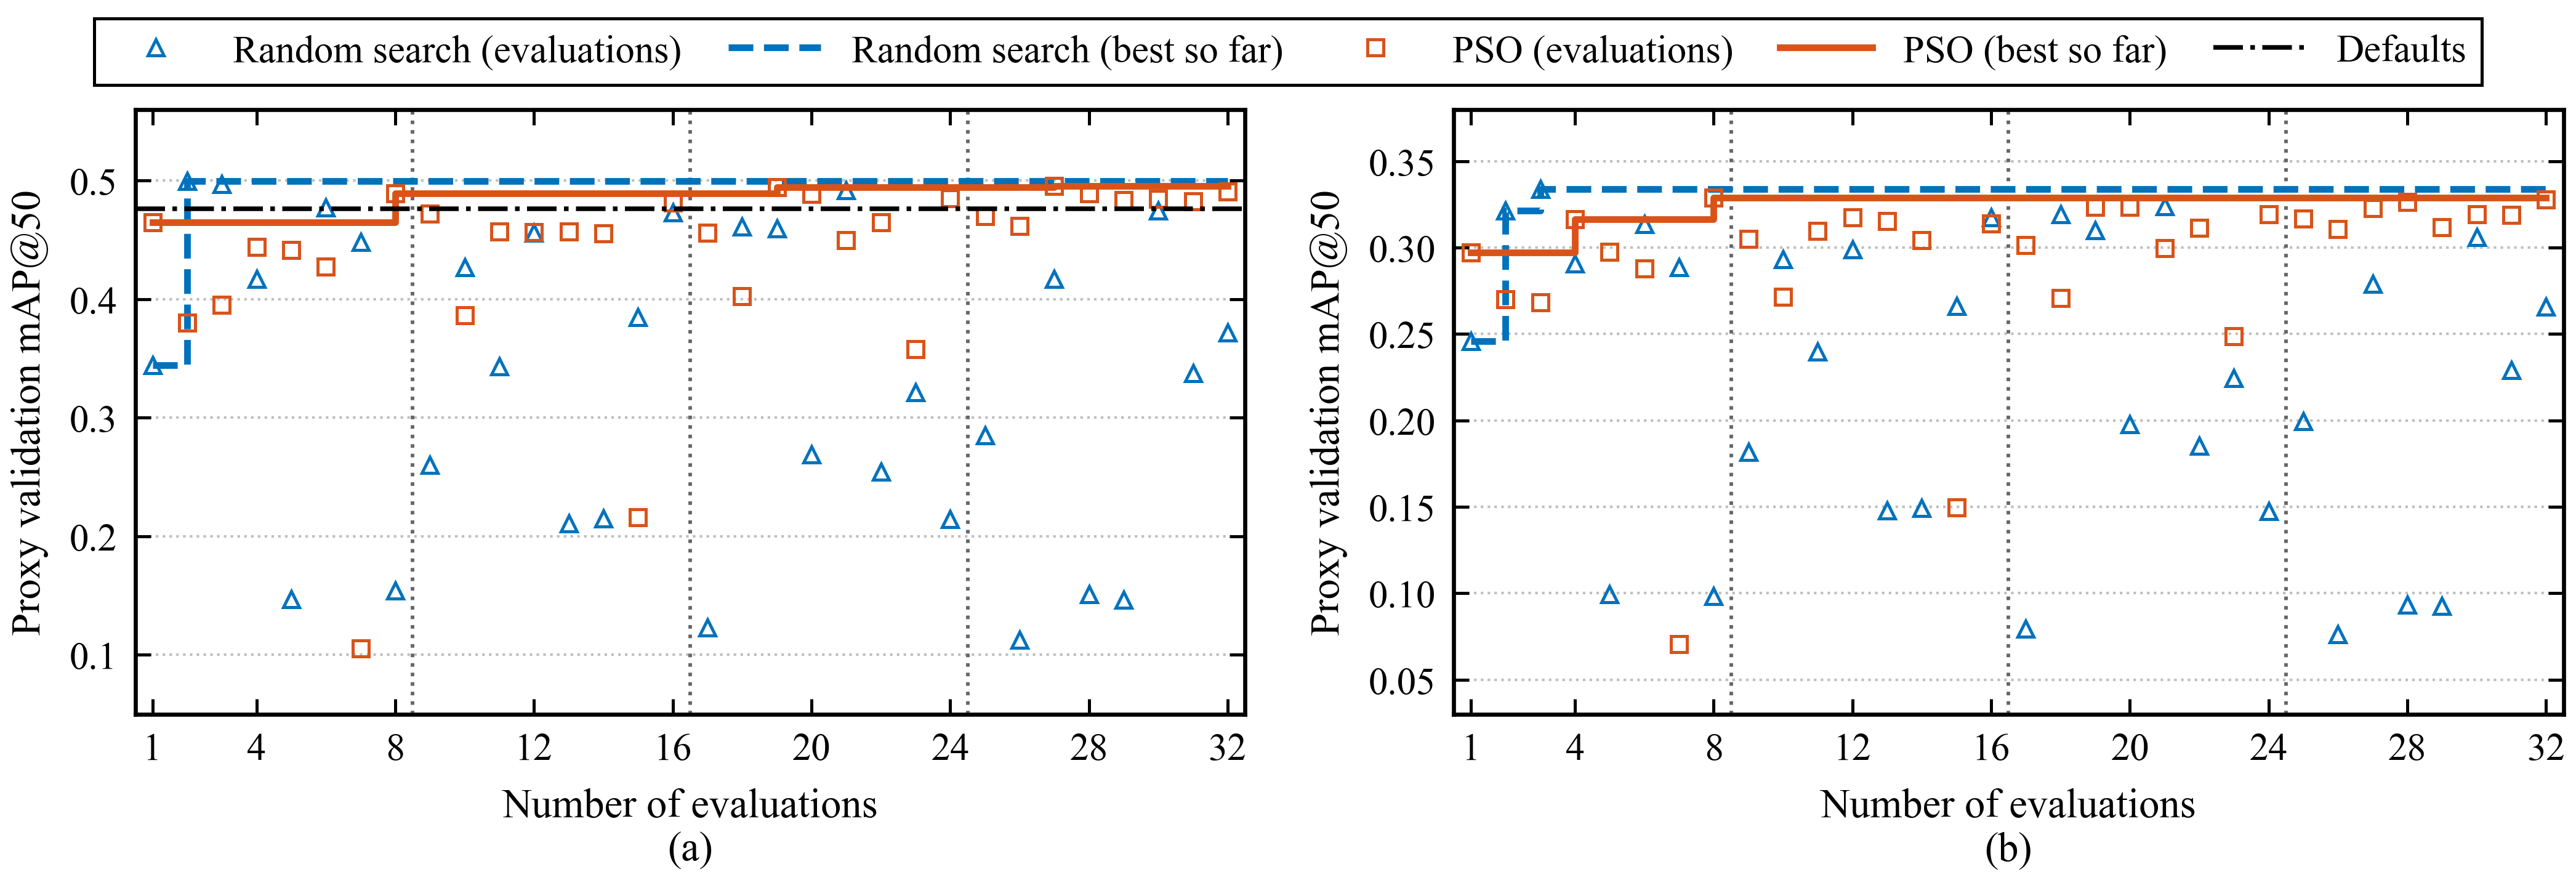
\includegraphics[width=\textwidth]{r_convergence.png}
\caption{Convergence of the two searches on the proxy fitness (validation \mapfifty after 12 epochs on 40\% of the training split) for (a) \genone and (b) \gentwo. Markers show the individual evaluations and lines show the best score obtained so far. The vertical dotted lines separate the four PSO rounds of eight particles each; random search has no rounds and is plotted in the order of sampling. The dash-dotted line in (a) is the score of the defaults on the same proxy, which was not run for \gentwo. The proxy scores of the two panels are not comparable since the validation sets, classes and image sizes are different.}
\label{fig:convergence}
\end{figure*}

In \gentwo, random search again found its best value early (0.3340 at evaluation~3). The best value of PSO, 0.3290, belonged to the last particle of round~1 and was not improved in the later rounds, whose best values were 0.3176, 0.3237 and 0.3279. The swarm nevertheless converged, with the round means rising from 0.267 to 0.286, 0.300 and 0.319 and the within-round standard deviation falling from 0.082 to 0.006. In both generations the mean proxy score of PSO over its 32 evaluations is higher than that of random search (0.437 versus 0.333 in \genone and 0.293 versus 0.226 in \gentwo). This is because the swarm places its later evaluations close to good points; it does not mean that better points were found. No proxy run of the defaults was made in \gentwo, so their position on the \gentwo proxy is not known.

\subsection{Generation~1 Test Results (Studio Data)}
\label{subsec:res-gen1}

The test results of the three \genone models on the 1,046 studio test images are given in Table~\ref{tab:gen1-test}. (The evaluator counts 7,415 boxes, whereas Table~\ref{tab:datasets} lists 7,413 because 2 zero-size boxes are omitted there.) The \mapfifty is 0.676 for Arm~A, 0.672 for Arm~B and 0.668 for Arm~C. For both metrics, the 95\% interval of every pairwise difference includes 0, and the largest difference is C$-$A with $-0.008$ [$-0.021$, $+0.007$]. The three arms are thus statistically tied on studio data. Going by the point estimates alone, the defaults are in fact first and PSO is last. Precision and recall are almost the same for the three arms. The validation scores agree with this picture. The defaults and PSO both reached 0.657, and random search, whose setting had the highest proxy score in \genone, reached the lowest value of 0.643.

\begin{table*}[!t]
\centering
\caption{\genone Test Results on the Studio Test Split (1,046 Images)}
\label{tab:gen1-test}
\footnotesize
\begin{tabular}{@{}lcccccc@{}}
\toprule
Arm & Val \mapfifty & Test \mapfifty [95\% CI] & Test \mapfiftyninetyfive [95\% CI] & P & R & ms/img \\
\midrule
A: Defaults & 0.657 & 0.676 [0.639, 0.722] & 0.474 [0.441, 0.518] & 0.747 & 0.581 & 31.4 \\
B: Random search & 0.643 & 0.672 [0.634, 0.717] & 0.475 [0.441, 0.519] & 0.746 & 0.587 & 38.3 \\
C: PSO & 0.657 & 0.668 [0.627, 0.717] & 0.471 [0.437, 0.516] & 0.747 & 0.586 & 31.7 \\
\bottomrule
\end{tabular}
\\[6pt]
\begin{tabular}{@{}lccccc@{}}
\toprule
Pair & $\Delta$\mapfifty [95\% CI] & $P(\Delta>0)$ & $\Delta$\mapfiftyninetyfive [95\% CI] & $P(\Delta>0)$ & Verdict \\
\midrule
B$-$A & $-0.004$ [$-0.016$, $+0.009$] & 0.30 & $+0.001$ [$-0.008$, $+0.010$] & 0.59 & not significant \\
C$-$A & $-0.008$ [$-0.021$, $+0.007$] & 0.16 & $-0.003$ [$-0.012$, $+0.007$] & 0.34 & not significant \\
C$-$B & $-0.004$ [$-0.015$, $+0.007$] & 0.24 & $-0.003$ [$-0.011$, $+0.004$] & 0.19 & not significant \\
\bottomrule
\end{tabular}
\\[2pt]
\parbox{\textwidth}{\footnotesize Val: best checkpoint on the validation split after 100 epochs. CIs: 1,000 paired bootstrap resamples of the test images. P and R at the confidence of maximum F1. ms/img: median batch-1 latency at 416~px on a laptop CPU (Intel Core Ultra~5 125H). $P(\Delta>0)$: share of resamples in which the first arm of the pair scored higher. A difference is significant only if its CI excludes 0.}
\end{table*}

Fig.~\ref{fig:gen1-perclass} shows the AP@50 for each class (without confidence intervals, see Section~\ref{subsec:eval}). On five of the six classes the arms are within 0.02 of each other. PLASTIC is the exception: PSO obtains 0.638, compared with 0.699 for Arm~A and 0.693 for Arm~B. PSO has the highest value on BIODEGRADABLE, GLASS and METAL. Since the three networks have the same architecture, the higher CPU latency of Arm~B in Table~\ref{tab:gen1-test} is most likely due to other load on the laptop at the time of measurement.

\begin{figure}[!t]
\centering
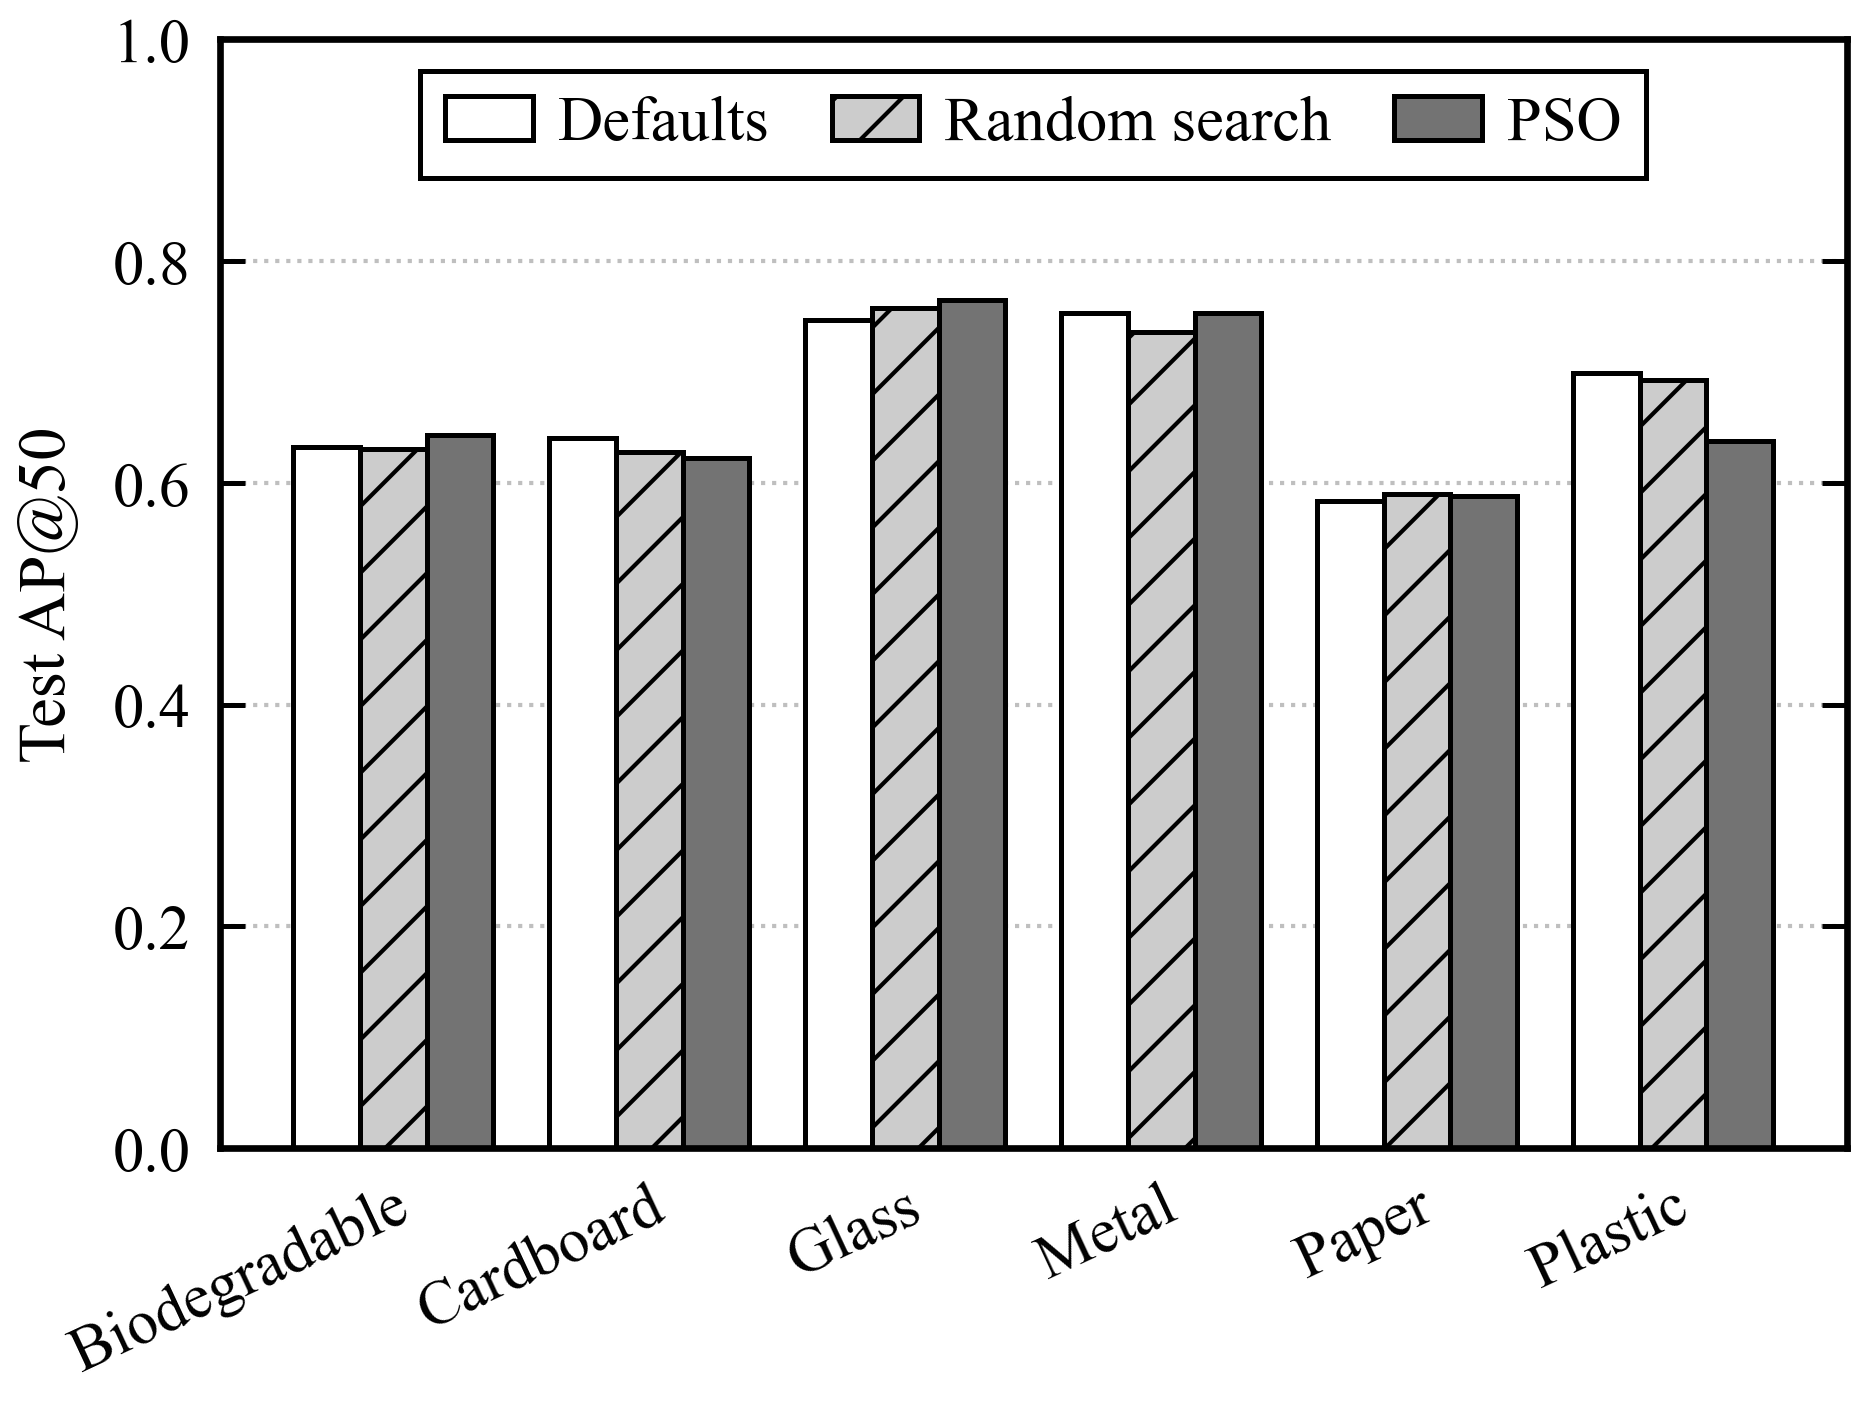
\includegraphics[width=\columnwidth]{r_gen1_per_class.png}
\caption{Per-class test AP@50 of the three \genone models on the studio test split. The number of test boxes as counted by the evaluator is 4,533 for BIODEGRADABLE, 392 for CARDBOARD, 822 for GLASS, 588 for METAL, 527 for PAPER and 553 for PLASTIC (7,415 in total, including 2 zero-size BIODEGRADABLE boxes). PSO is lowest on PLASTIC, and on the other classes the arms are within 0.02 of each other.}
\label{fig:gen1-perclass}
\end{figure}

\subsection{Generation~2 Test Results (Mixed Data)}
\label{subsec:res-gen2}

Table~\ref{tab:gen2-test} lists the \gentwo test results for the complete test split and for each domain. On the complete split, the \mapfifty is 0.479 for the defaults, 0.497 for random search and 0.500 for PSO. Both tuned arms are significantly better than the defaults (B$-$A $+0.017$ [$+0.006$, $+0.030$] and C$-$A $+0.020$ [$+0.011$, $+0.032$]). PSO and random search, on the other hand, cannot be distinguished (C$-$B $+0.003$ [$-0.008$, $+0.015$]). The intervals of the individual arms overlap to a large extent. The gains are detected only because the paired bootstrap removes the variation in image difficulty, which is common to all three models. For \mapfiftyninetyfive the verdicts are the same as for \mapfifty in all cases. On the validation split random search was ahead of PSO (0.473 versus 0.466), but on the test split the two are tied.

Out of the 8,192 test boxes, 7,413 come from studio images. The studio test set alone, i.e., the 1,046 test images of \genone, leads to the same conclusion: B$-$A ($+0.024$) and C$-$A ($+0.019$) are significant and C$-$B ($-0.005$) is not. The only place where PSO and random search differ significantly is the Indian test set, where all the scores are close to zero (Section~\ref{subsec:res-domain}).

\begin{table*}[!t]
\centering
\caption{\gentwo Test Results per Test Set: \mapfifty and \mapfiftyninetyfive [95\% CI] per Arm, and Pairwise Differences in \mapfifty}
\label{tab:gen2-test}
\footnotesize
\begin{tabular}{@{}lcccc@{}}
\toprule
 & All & Studio & Real-world & India (DWSD) \\
 & 1,514 img., 8,192 boxes & 1,046 img., 7,413 boxes & 468 img., 779 boxes & 700 img., 4,502 boxes \\
\midrule
\multicolumn{5}{@{}l}{\textit{Test \mapfifty [95\% CI]}} \\
A: Defaults & 0.479 [0.453, 0.513] & 0.571 [0.529, 0.619] & 0.310 [0.278, 0.440] & 0.027 [0.024, 0.031] \\
B: Random search & 0.497 [0.471, 0.531] & 0.595 [0.557, 0.639] & 0.298 [0.271, 0.407] & 0.023 [0.021, 0.027] \\
C: PSO & 0.500 [0.474, 0.534] & 0.590 [0.550, 0.635] & 0.310 [0.279, 0.415] & 0.027 [0.024, 0.031] \\
\midrule
\multicolumn{5}{@{}l}{\textit{$\Delta$\mapfifty [95\% CI] (bold: significant, CI excludes 0)}} \\
B$-$A & $\mathbf{+0.017}$ [$+0.006$, $+0.030$] & $\mathbf{+0.024}$ [$+0.009$, $+0.038$] & $-0.012$ [$-0.118$, $+0.053$] & $\mathbf{-0.003}$ [$-0.006$, $-0.001$] \\
C$-$A & $\mathbf{+0.020}$ [$+0.011$, $+0.032$] & $\mathbf{+0.019}$ [$+0.005$, $+0.033$] & $+0.001$ [$-0.111$, $+0.065$] & $+0.000$ [$-0.003$, $+0.003$] \\
C$-$B & $+0.003$ [$-0.008$, $+0.015$] & $-0.005$ [$-0.018$, $+0.009$] & $+0.013$ [$-0.015$, $+0.036$] & $\mathbf{+0.003}$ [$+0.001$, $+0.006$] \\
\midrule
\multicolumn{5}{@{}l}{\textit{Test \mapfiftyninetyfive [95\% CI]}} \\
A: Defaults & 0.329 [0.309, 0.358] & 0.386 [0.356, 0.425] & 0.254 [0.224, 0.371] & 0.015 [0.013, 0.018] \\
B: Random search & 0.342 [0.322, 0.372] & 0.404 [0.374, 0.442] & 0.238 [0.213, 0.330] & 0.013 [0.012, 0.015] \\
C: PSO & 0.343 [0.323, 0.374] & 0.398 [0.367, 0.439] & 0.248 [0.220, 0.336] & 0.015 [0.013, 0.017] \\
\bottomrule
\end{tabular}
\\[2pt]
\parbox{\textwidth}{\footnotesize All test sets were scored once, at 640~px, with 1,000 paired bootstrap resamples per test set. ``All'' is the whole \gentwo test split (studio plus real-world); India is DWSD, used for testing only. The \mapfiftyninetyfive differences give the same verdict as the \mapfifty differences in every cell. Validation \mapfifty: A 0.454, B 0.473, C 0.466.}
\end{table*}

Looking at the individual classes on the complete split, PSO has the highest AP@50 on five of the seven classes and random search on BIODEGRADABLE and PLASTIC, while the defaults are not the best on any class. The OTHER class is very weak in all arms (AP@50 of 0.050--0.063), and all of its 132 test boxes are in the real-world images. Precision increases from 0.549 (A) to 0.563 (B) and 0.582 (C), and recall increases from 0.445 (A) to 0.470 for both tuned arms. The median latency on the T4 at 640~px lies between 8.1 and 8.7~ms per image.

\subsection{Domain Gap}
\label{subsec:res-domain}

When averaged over the three \gentwo arms, the test \mapfifty drops from about 0.59 on studio images to 0.31 on real-world images and 0.03 on Indian images (Fig.~\ref{fig:domains}). For each arm, the real-world score is approximately half of the studio score.

\begin{figure}[!t]
\centering
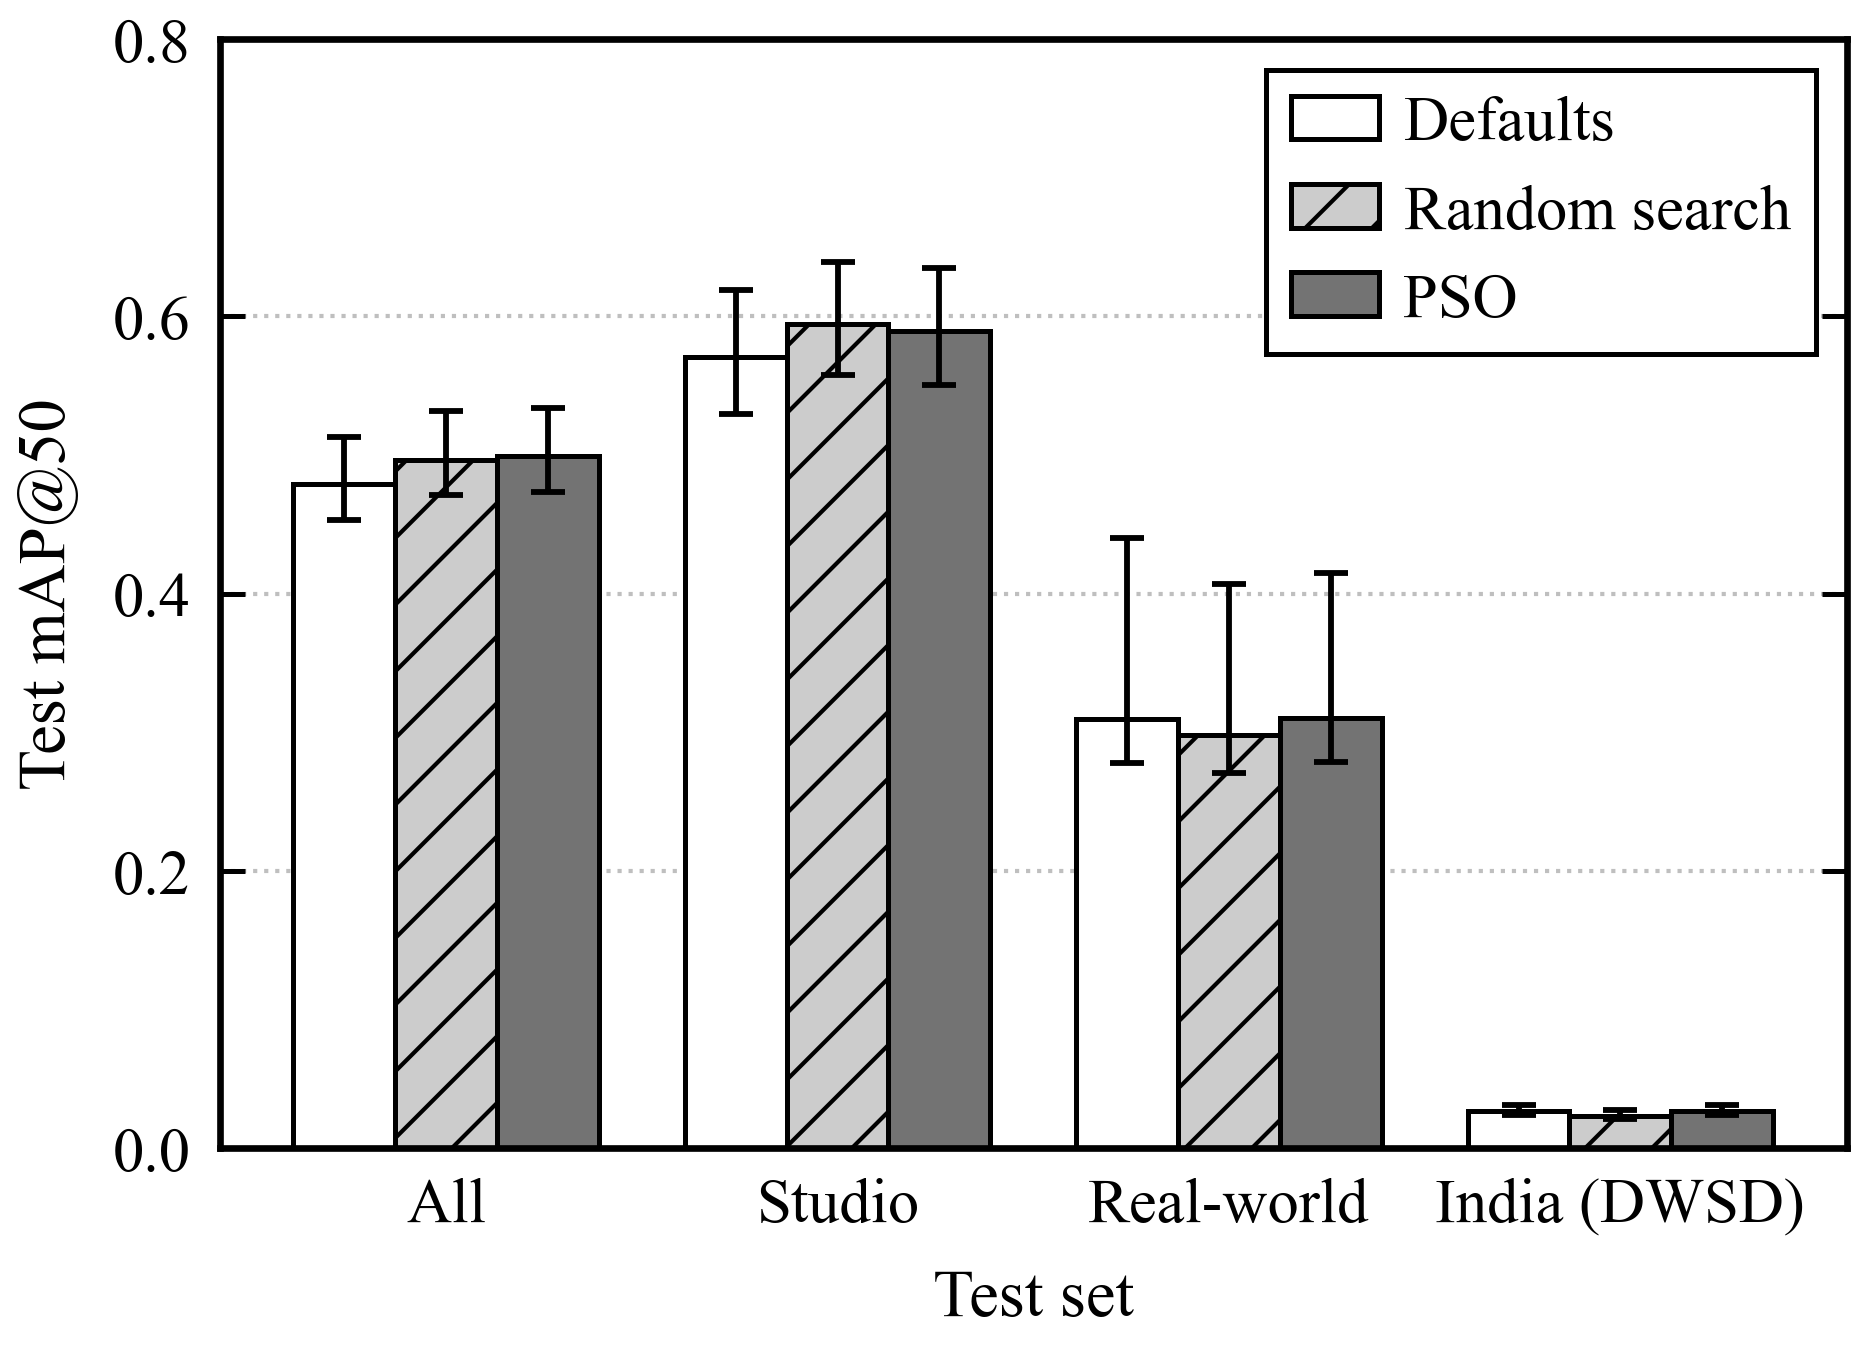
\includegraphics[width=\columnwidth]{r_domains.png}
\caption{Test \mapfifty of the three \gentwo models on each test set. The error bars are 95\% paired-bootstrap confidence intervals. ``All'' (1,514 images) combines the studio (1,046) and real-world (468) test images, and India (DWSD, 700 images) was used for testing only. The real-world intervals are asymmetric because that set has only one BIODEGRADABLE box.}
\label{fig:domains}
\end{figure}

On the 468 real-world test images from TACO and HITL, none of the pairwise differences is significant (Table~\ref{tab:gen2-test}). The intervals are wide and asymmetric, and the reason is that BIODEGRADABLE has just one box in this set. Depending on whether a resample omits or repeats that image, the AP of this class changes sharply, and this class makes up one seventh of the mean. On that single box the arms obtain an AP@50 of 0.249 (A), 0.020 (B) and 0.003 (C). The intervals of B$-$A and C$-$A are 0.17 to 0.18 wide, so differences of the magnitude seen on studio images (around 0.02) cannot be resolved on this set.

On the 700 DWSD images from India, all three models fail. The \mapfifty is between 0.023 and 0.027, precision is 0.070--0.075 and recall is 0.043--0.047. Only PLASTIC (0.089--0.101) and PAPER (0.028--0.035) have an AP@50 above 0.01. The defaults and PSO are both significantly above random search and are not different from each other. For \mapfiftyninetyfive, the two significant differences are B$-$A $-0.002$ [$-0.003$, $-0.001$] and C$-$B $+0.002$ [$+0.000$, $+0.003$]; the lower bound of the latter is 0.0004 before rounding. Since these differences are of a few thousandths on scores that are nearly zero, they have no practical significance.

Four reasons for this failure can be identified from the data (Section~\ref{subsec:datasets}). First, no Indian image was used in training, search or model selection. Second, the DWSD images appear to be augmented (rotated, with black corners and color tints) and look unlike any of the training images. Third, the DWSD boxes are derived from mask regions. Touching items of a class are merged into one large box, which overlaps poorly with per-item detections, so that even correct detections are often counted as misses. Fourth, the mapping of mask values to classes was inferred from the images, and six of the fifteen values are uncertain. The India score is therefore a measure of the difference in labeling style as much as of the models. Fig.~\ref{fig:samples} shows the output of the three models for two studio, two real-world and two DWSD test images. Both real-world images contain eight objects. In the first one each model finds three objects at most, and in the second none. On the DWSD images each model predicts at most one box, whereas the ground truth has 4 and 19 boxes. In the first DWSD image, all three models draw a box around the region which the ground truth labels as PAPER, but classify it as PLASTIC.

\begin{figure*}[p]
\centering
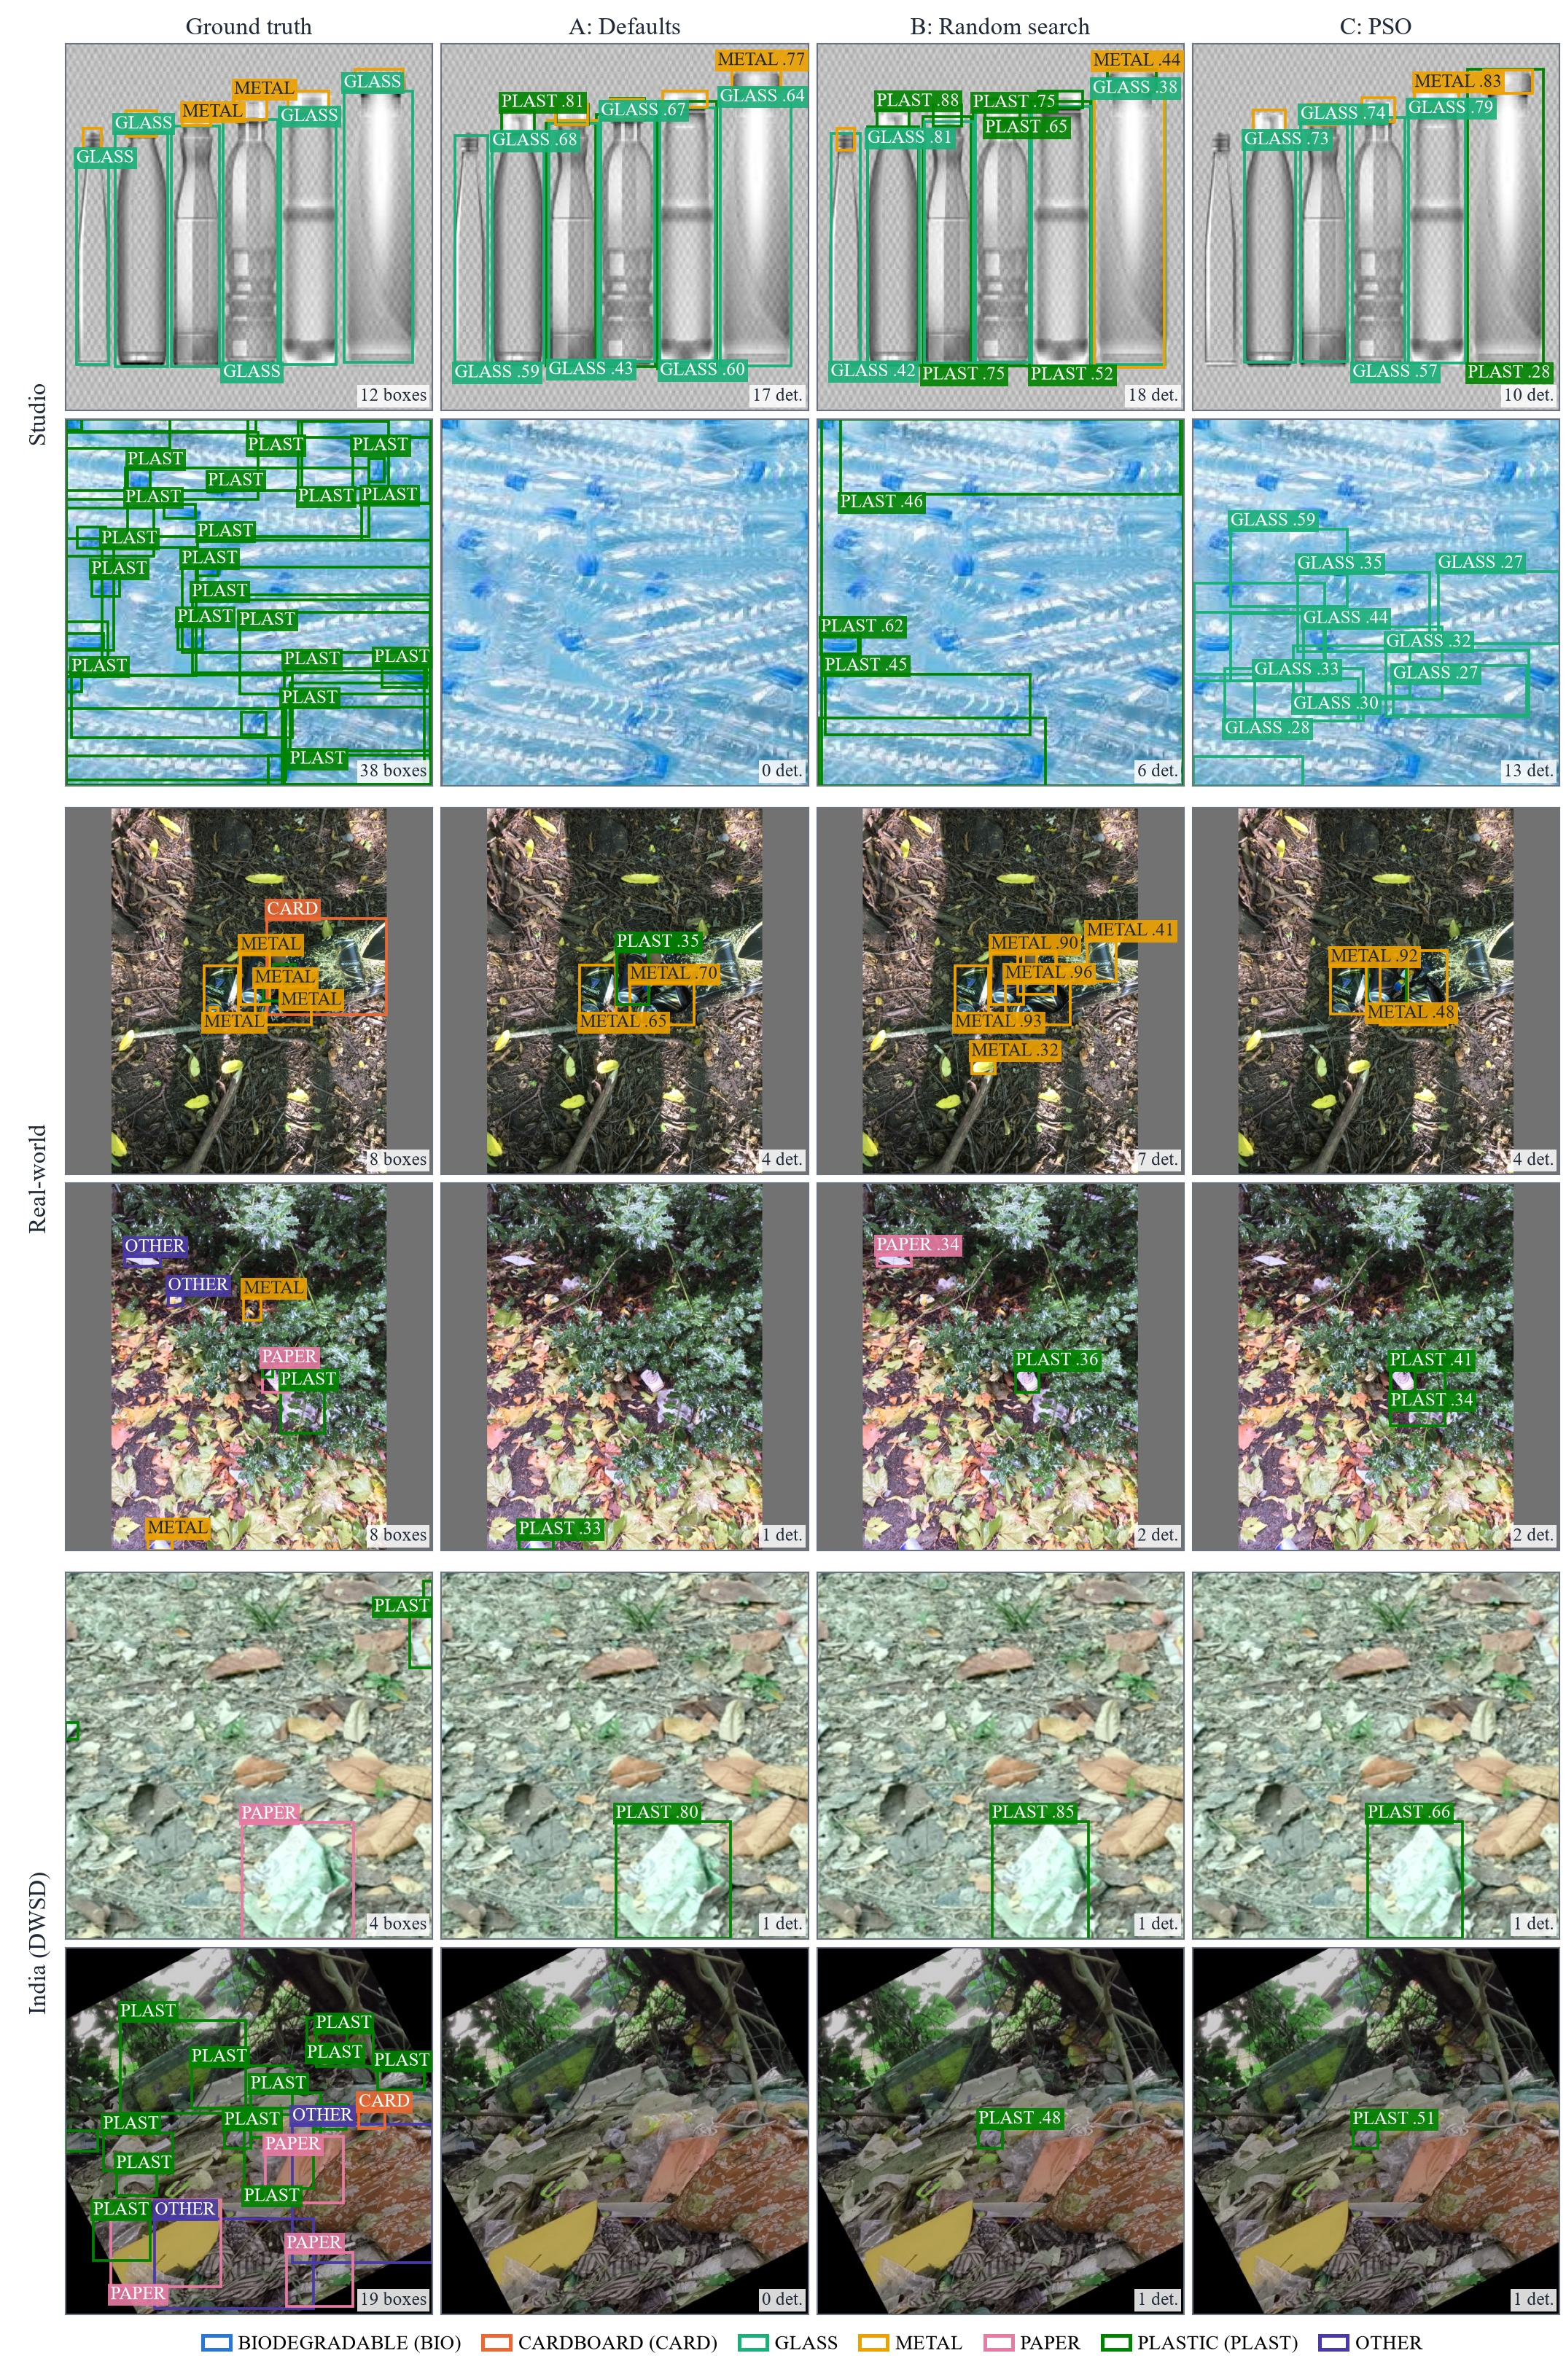
\includegraphics[width=0.85\textwidth]{r_samples.jpg}
\caption{Detections of the three \gentwo models on two studio, two real-world and two Indian (DWSD) test images, next to the ground truth. The images were not picked by hand: for each test set, the images having at least three ground-truth boxes were shuffled with seed 0 and the first two are shown. All models were given the same images at 640~px with a confidence threshold of 0.25 and an NMS IoU of 0.7; the real-world rows show the predictions recorded in the per-image analysis of Fig.~\ref{fig:best}. Each box is marked with its class and, for predictions, its confidence, and a label is omitted if it would cover another one. The number of ground-truth boxes or detections is given in the corner of each panel. These examples are only illustrative; for the quantitative results see Table~\ref{tab:gen2-test} and Fig.~\ref{fig:domains}. The DWSD ground-truth boxes come from mask regions, so touching items of one class can merge into one box.}
\label{fig:samples}
\end{figure*}

As mentioned before, the two generations have different classes, image sizes and training data, and Tables~\ref{tab:gen1-test} and~\ref{tab:gen2-test} cannot be read as one benchmark. In Table~\ref{tab:g1g2}, all six final models are therefore evaluated on the same studio and real-world test images using only the six shared classes (Section~\ref{subsec:eval}). On the real-world images, every \gentwo arm is significantly better than every \genone arm, with a \mapfifty of 0.338--0.353 against 0.038--0.096, which is roughly four to nine times higher. On the studio images the situation is reversed, and every \genone arm is significantly better than every \gentwo arm by 0.074 to 0.105. Within a generation, none of the real-world differences is significant (e.g., \genone C$-$A $+0.048$ [$-0.020$, $+0.163$] and \gentwo C$-$B $+0.013$ [$-0.019$, $+0.042$]), and the studio verdicts are the same as in Tables~\ref{tab:gen1-test} and~\ref{tab:gen2-test}. The value of 0.096 for \genone C and its wide interval are mainly caused by the single real-world BIODEGRADABLE box, on which this model has an AP@50 of 0.332. The real-world scores of \gentwo are higher here than in Table~\ref{tab:gen2-test} (0.353 against 0.310 for Arm~A) only because OTHER is excluded from the mean. As a sanity check, \genone reproduces its own studio test result to within 0.0004 \mapfifty.

\begin{table}[!t]
\centering
\caption{\genone versus \gentwo on the Same Test Images: Test \mapfifty [95\% CI] on the Six Shared Classes}
\label{tab:g1g2}
\footnotesize
\begin{tabular}{@{}lcc@{}}
\toprule
Model (px) & Real-world (468 img.) & Studio (1,046 img.) \\
\midrule
G1 A (416) & 0.047 [0.038, 0.080] & 0.676 [0.641, 0.719] \\
G1 B (416) & 0.038 [0.031, 0.069] & 0.672 [0.636, 0.716] \\
G1 C (416) & 0.096 [0.041, 0.214] & 0.669 [0.628, 0.716] \\
\midrule
G2 A (640) & 0.353 [0.315, 0.504] & 0.571 [0.529, 0.619] \\
G2 B (640) & 0.338 [0.304, 0.473] & 0.595 [0.557, 0.639] \\
G2 C (640) & 0.352 [0.315, 0.485] & 0.590 [0.550, 0.635] \\
\midrule
$\Delta$ G2$-$G1 & $+0.243$ to $+0.315$ & $-0.105$ to $-0.074$ \\
\bottomrule
\end{tabular}
\\[2pt]
\parbox{\columnwidth}{\footnotesize G1, G2: \genone, \gentwo; each model was scored once at its own training image size (px). Real-world: 647 boxes after removing OTHER, with a single BIODEGRADABLE box; studio: 7,413 boxes, no OTHER. CIs: 1,000 paired bootstrap resamples per test set. $\Delta$: range over all nine G2$-$G1 pairs, every one significant; e.g., real-world G2 B$-$G1 C $+0.243$ [$+0.134$, $+0.418$], studio G2 A$-$G1 A $-0.105$ [$-0.125$, $-0.084$]. On the five real-world classes with more than one box, \gentwo scores 0.239--0.618 AP@50 and \genone 0.008--0.117.}
\end{table}

To understand where the \gentwo models do succeed on real-world photographs, we analyzed the 468 real-world test images one by one. An image is considered fully correct if every ground-truth object is matched by a detection of the same class with IoU $\geq 0.5$ and no detection remains unmatched. Matching is greedy in the order of decreasing confidence, with a confidence threshold of 0.25. The models are fully correct on 166 (A), 168 (B) and 170 (C) images, i.e., 35 to 36\% of the set, and all three are correct on the same 111 images. Nearly all of these are photographs with a single object. Of the 375 images with one object, the models are fully correct on 164 to 167. Of the 47 images with two objects, they are correct on 1 to 4, and of the 46 images with three or more objects, on none. Fig.~\ref{fig:best} shows the most favorable cases, which were selected by a fixed rule. No image with three or more objects is fully correct for all three models, and only one image with two objects is. The rule therefore falls back on the two images with at least two objects that are labeled fully correctly by at least two models. One of them is a close-up on a plain background, which is close to studio conditions. In short, the models can deal with an isolated item in a real scene but not with a cluttered scene containing several items.

\begin{figure*}[!t]
\centering
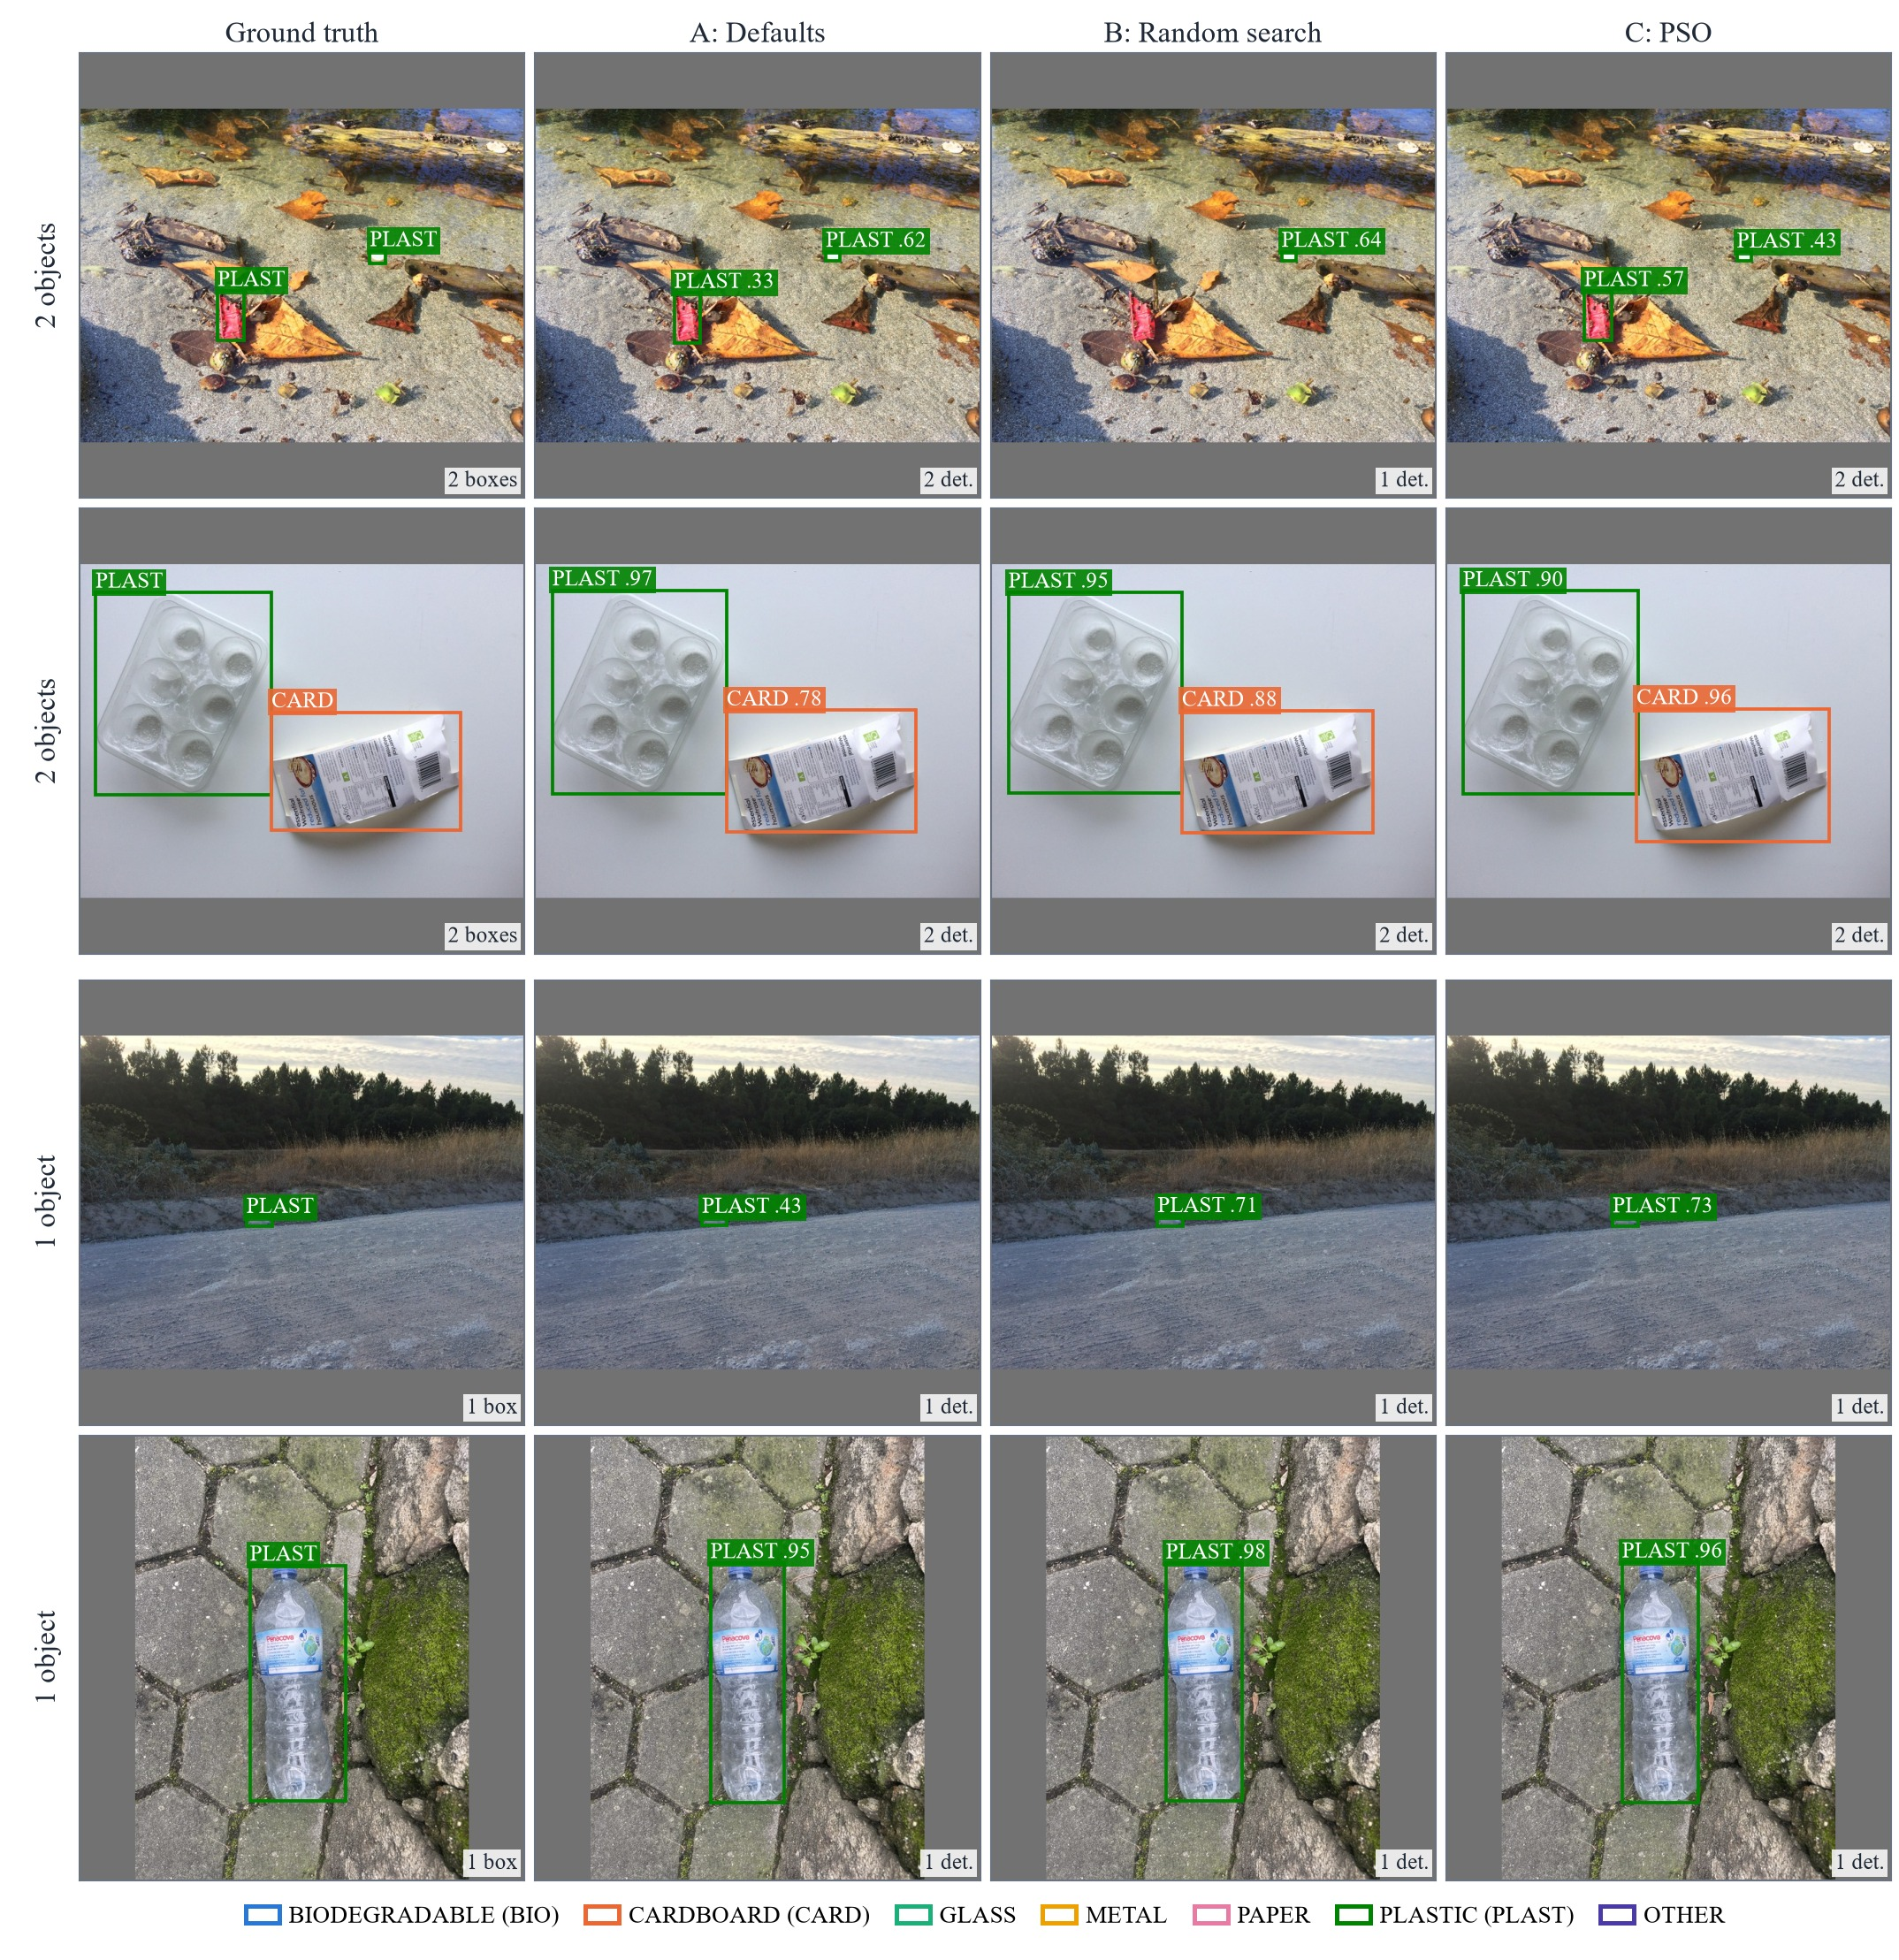
\includegraphics[width=0.8\textwidth]{r_best.jpg}
\caption{Success cases on real-world test images. These are the most favorable examples and are not representative of the whole set. Rows 1--2: the only real-world test images with at least two objects that at least two of the three \gentwo models label fully correctly (every object found with the right class, no false detection); no image with three or more objects qualifies, and random search (B) misses one object in the first. Rows 3--4: the first two of the 110 single-object images that all three models label fully correctly, in a random order with seed 0. Confidence threshold 0.25, NMS IoU 0.7, 640~px. For scale, each model is fully correct on 166--170 of the 468 real-world test images, on 164--167 of the 375 single-object images and on none of the 46 images with three or more objects.}
\label{fig:best}
\end{figure*}

\subsection{Compute Cost}
\label{subsec:res-cost}

The GPU time recorded for each run on the Tesla T4 is given in Table~\ref{tab:compute}. Only the training time is counted; setup, copying of data and idle time are excluded. When the search is included, each tuned arm costs about 2.7 to 2.8 times the GPU time of Arm~A, which requires no search. The budget was equal in terms of evaluations but not in terms of time. A proxy training took 214.3~s on average for PSO and 238.7~s for random search in \genone, and 285.5~s and 259.0~s in \gentwo. The most expensive item in \genone was the proxy-validity check, in which the eight 40-epoch medium runs accounted for 3.84 of the 4.36 hours. In \gentwo, about 24 additional GPU-hours were wasted when two sessions froze and remained idle until the 12-hour limit of the platform was reached; these hours are not part of the totals. The one-time test evaluation took 283.1~s on the laptop CPU in \genone and 220.6~s on the T4 for the four test sets of \gentwo.

\begin{table}[!t]
\centering
\caption{Recorded GPU Time per Run (Hours, One Tesla T4)}
\label{tab:compute}
\footnotesize
\begin{tabular}{@{}lcc@{}}
\toprule
Run & \genone & \gentwo \\
\midrule
Proxy-validity check (16 runs) & 4.36 & not run \\
PSO search (32 proxy trainings) & 1.91 & 2.54 \\
Random search (32 proxy trainings) & 2.12 & 2.30 \\
Arm~A full training (100 epochs) & 1.18 & 1.56 \\
Arm~B full training (100 epochs) & 1.15 & 2.07 \\
Arm~C full training (100 epochs) & 1.45 & 1.60 \\
\midrule
Total recorded & 12.18 & 10.06 \\
\bottomrule
\end{tabular}
\\[2pt]
\parbox{\columnwidth}{\footnotesize Sums of the recorded training wall-clock times. The \gentwo random search and Arm~C training were resumed after a session froze (Arm~C after epoch 55); their idle time, about 24 GPU-hours in total, is not included.}
\end{table}
